\appendix
%\chapter{Hyperparameter hierarchy example}
%	\label{ap:hyperparam_hierarchy}
%
%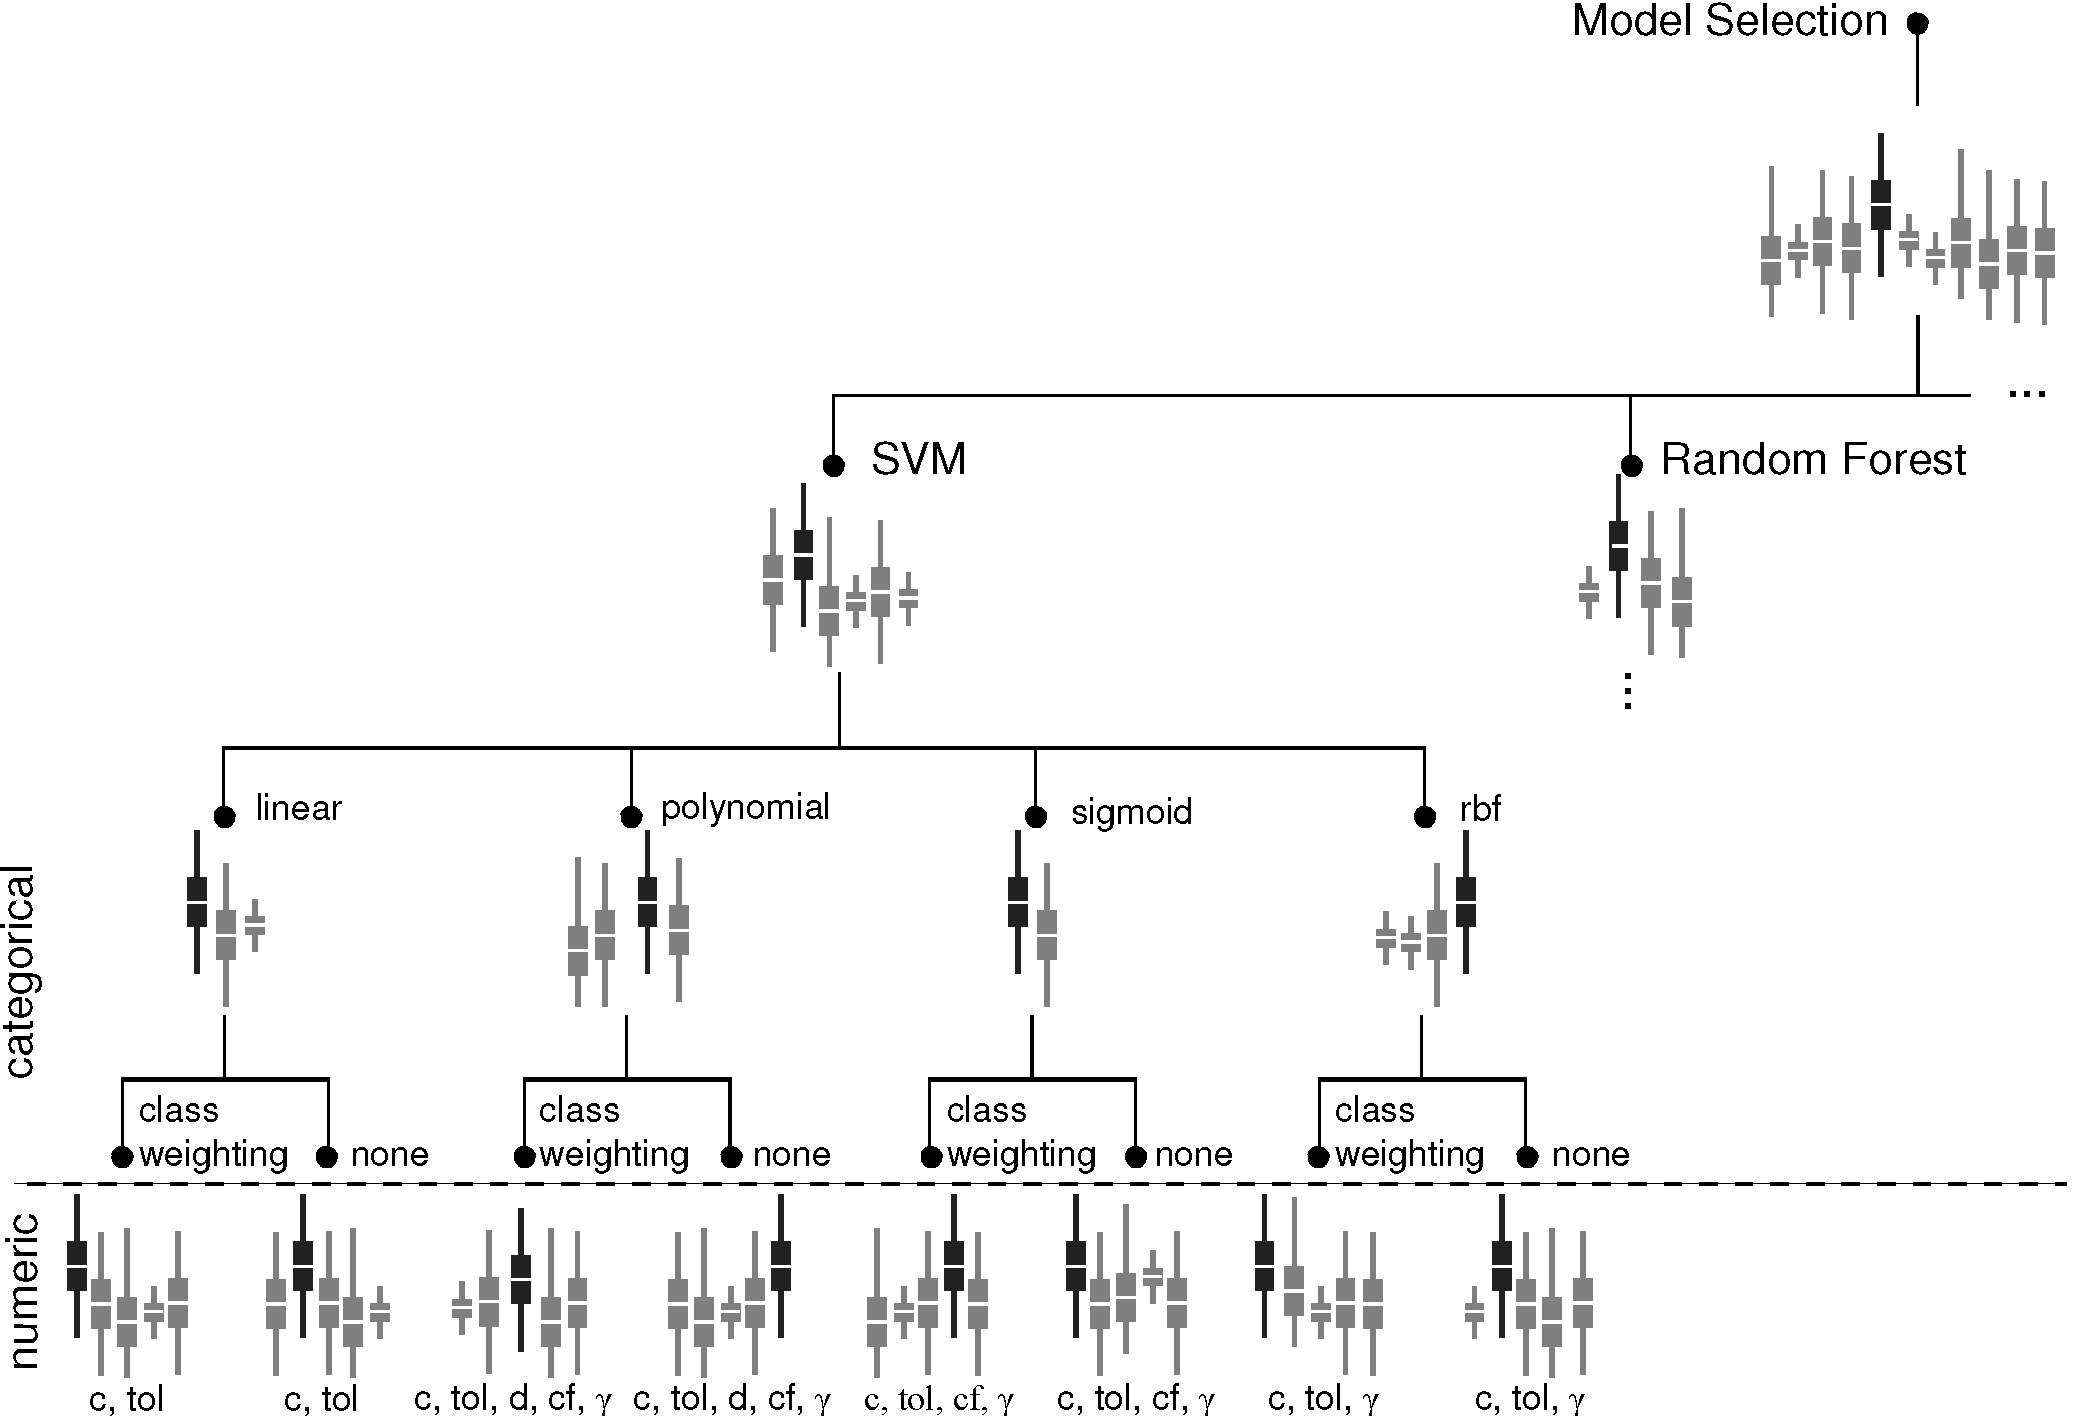
\includegraphics[width=\textwidth]{tree}

\chapter{Supervised machine learning algorithms}

The following SML algorithms are used in this work:

\begin{tabularx}{\textwidth}{l X}
Name & Description\\
\hline

%\texttt{KNN} & Assigns the class with most representatives out of the $k$ nearest neighbors of an instance.\\
%\texttt{RadiusNeighbors} & Assigns the class with most representatives within a radius.\\
%\texttt{NearestCentroid} & Assigns the class of the centroid of the nearest cluster.\\
%\texttt{StochasicGradientDescent} & \\
%\texttt{LogisticRegression} & Applies a logistic (sigmoid) function on a linear combination of
%the features to decide the class of an instance.\\
%\texttt{SVM} & Divides the feature space by using support vectors given by different kernel
%functions (libSVM implementation), and assigns different classes to instances in each subdivision.\\
%\texttt{LinearSVM} & Uses linear support vectors to divide the feature space and assign classes
%to elements belonging to the same subdivision (libLinear implementation).\\
%\texttt{NuSVM} & SVM implementation that controls the number of support vectors.\\
%\texttt{DecisionTree} & Applies iterative decisions on the different dimensions of the feature space
%to assign classes.\\
%\texttt{RandomForest} & Fits a number of decision trees to subsets of the data and uses averaging of
%such models to prevent overfitting.\\
%\texttt{ExtraTreeEnsemble} & \\
%\texttt{Ridge} & Assigns classes using Ridge regression.\\
%\texttt{LinearDiscriminant} & Linear discriminant analysis.\\
%\texttt{QuadraticDiscriminant} & Quadratic discriminant analysis.\\
%\texttt{GradientBoosting} & \\
%\texttt{PassiveAggressive} & \\
%\texttt{GaussianNB} & \\
%\end{tabularx}


\texttt{KNN} & $k$-nearest neighbors classifier.\\
\texttt{RadiusNeighbors} & Votes among neighbors within a certain radius. \\
\texttt{NearestCentroid} & Assigns the class of the centroid of the nearest cluster.\\
\texttt{StochasicGradientDescent} & Stochastic Gradient Descent classifier.\\
\texttt{LogisticRegression} & Logistic function applied on a linear combination of features.\\
\texttt{SVM} & Support Vector Machine (libSVM implementation).\\
\texttt{LinearSVM} & Linear SVM (libLinear implementation).\\
\texttt{NuSVM} & Nu-Support Vector Machine.\\
\texttt{DecisionTree} & Decision tree classification.\\
\texttt{RandomForest} & Average of multiple decision trees on subsets of the data.\\
\texttt{ExtraTreeEnsemble} & Random forest with randomized decision trees.\\
\texttt{Ridge} & Least squares regression with L2 loss.\\
\texttt{LinearDiscriminant} & Linear discriminant analysis.\\
\texttt{QuadraticDiscriminant} & Quadratic discriminant analysis.\\
\texttt{GradientBoosting} & An ensemble of regression tree classifiers.\\
\texttt{PassiveAggressive} & Passive Aggressive classifier.\\
\texttt{GaussianNB} & Gaussian Na\"ive Bayes classifier\\
\end{tabularx}


\chapter{Datasets}

\begin{tabularx}{\textwidth}{X r r r}
\bf Standard datasets& \bf Instances & \bf Features & \bf Classes\\
\hline

balance-scale & 625 & 4 & 3\\
blood-transfusion  748 & 4 & 2\\
cmc & 1473 & 9 & 3\\
dermatology & 366 & 34 & 6 \\
diabetes & 768 & 8 & 2\\
haberman & 306 & 4 & 2\\
heart-statlog & 270 & 13 & 2 \\
ionosphere & 351 & 34 & 2\\
iris & 150 & 4 & 3\\
kdd\_synthetic\_control & 600 & 60 & 6\\
letter & 20000 & 16 & 26\\
liver-disorders & 345 & 7 & 2 \\
mfeat-factors & 2000 & 649 & 10 \\
mfeat-fourier & 2000 & 649 & 10 \\
mfeat-karhunen & 2000 & 649 & 10 \\
mfeat-morphological  & 2000 & 649 & 10 \\
mfeat-pixel & 2000 & 649 & 10 \\
mfeat-zernike  & 2000 & 649 & 10 \\
optdigits & 3823 & 64 & 10 \\
page-blocks & 5473 & 10 & 5 \\
pendigits & 7494 & 16 & 10 \\
segment-test & 2100 & 19 & 7\\
sonar & 208 & 60 & 2\\
spambase & 4601 & 57 & 2\\
tae & 151 & 5 & 3 \\
vehicle & 946 & 18 & 4\\
vowel & 990 & 14 & 11 \\
waveform-5000 & 5000 & 21 & 3\\
wine & 178 & 13 & 3 \\
\end{tabularx}
\clearpage

\begin{tabularx}{\textwidth}{X r r r}
\bf Biological datasets& \bf Instances & \bf Features & \bf Classes\\
\hline
HK2\_Standardized & 1441 & 25 & 6 \\
Huotari500\_Standardized & 502 & 25 & 4 \\
Meier500\_Standardized & 500 & 27 & 5 \\
so & 721 & 160 & 6\\
WildMain500\_Standardized & 500 & 25 & 5 \\
yeast & 1484 & 8 & 10 \\
colonTumor & 62 & 2000 & 2\\
\end{tabularx}

These datasets are available at \url{http://repository.seasr.org/Datasets/}.
